\documentclass[a4paper,11pt]{article}
\addtolength{\textwidth}{1.5in}
\addtolength{\hoffset}{-0.75in}
\usepackage{subfigure}
%\addtolength{\textheight}{0.5in}
%\addtolength{\voffset}{-0.25in}
\usepackage{rotating}
\usepackage{comment}
\usepackage{english}
\usepackage[T1]{fontenc}
\usepackage[latin1]{inputenc}
\usepackage{hyperref}
\usepackage{amsmath}
\usepackage{graphicx}
\usepackage{fancyhdr}
\usepackage{graphicx}
\usepackage{minipage}
\usepackage{listings}
\lstset{language=Matlab}
\pagestyle{fancy}
\lhead{}
\chead{}
\rhead{}
\lfoot{}
\cfoot{}
\rfoot{\thepage}
\title{\textbf{\huge{Artificial neural networks - Lab 1}}}
%\author{Magnus Raunio, 900531-5131}
\selectlanguage{english}

\begin{document}

\maketitle

\section{One layered neural network with delta rule}

For the one layered network we used the delta rule which minimizes the total error for the classifier, although not in the sense that it minimizes the number of incorrectly classified instances, but that the error/distance from the separating line to the instances becomes minimum. Below you can see the matrix transformations for the 

\vspace{5cm}
\begin{figure}[h!]
\caption{The one layer neural network layout and it's matrix transformation.}
\end{figure}

In figure \ref{fig:linear1:sub1} you can see the linearly seperable data generated to test the network and in figure \ref{fig:linear1:sub2} you can see the separating line that the neural network finds. In figure \ref{fig:linear1:sub3} we can also see the way the seperating line converges to it's final values. The steps to adjust the weight matrix decrease as the neural network converges as can be seen by the decreasing angle/distance between the seperating lines.

\begin{figure}[h!]
%\centering
\subfigure[Seperable data]{
    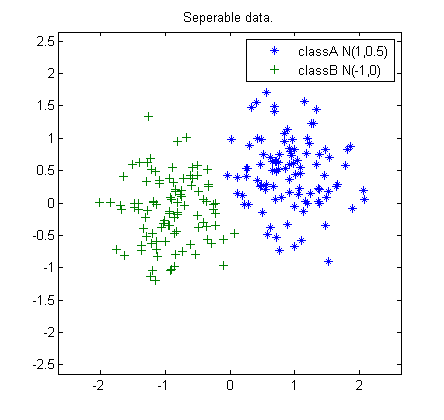
\includegraphics[width=0.5\linewidth]{lab1/seperabledata.png}
    \label{fig:linear1:sub1}
}
\subfigure[Seperaing line between data]{
    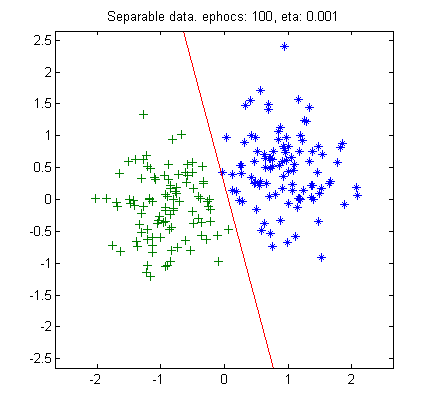
\includegraphics[width=0.5\linewidth]{lab1/linearsepdatalast.png}
    \label{fig:linear1:sub2}
}
\subfigure[The movement of the seperating line to it's final position.]{
    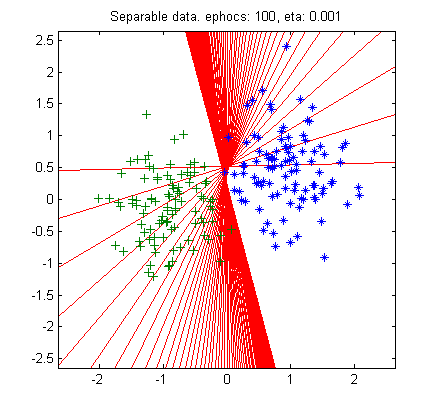
\includegraphics[width=0.5\linewidth]{lab1/linearsepdataall.png}
    \label{fig:linear1:sub3}
}
\subfigure[The error function we're minmizing with the delta rule.]{
    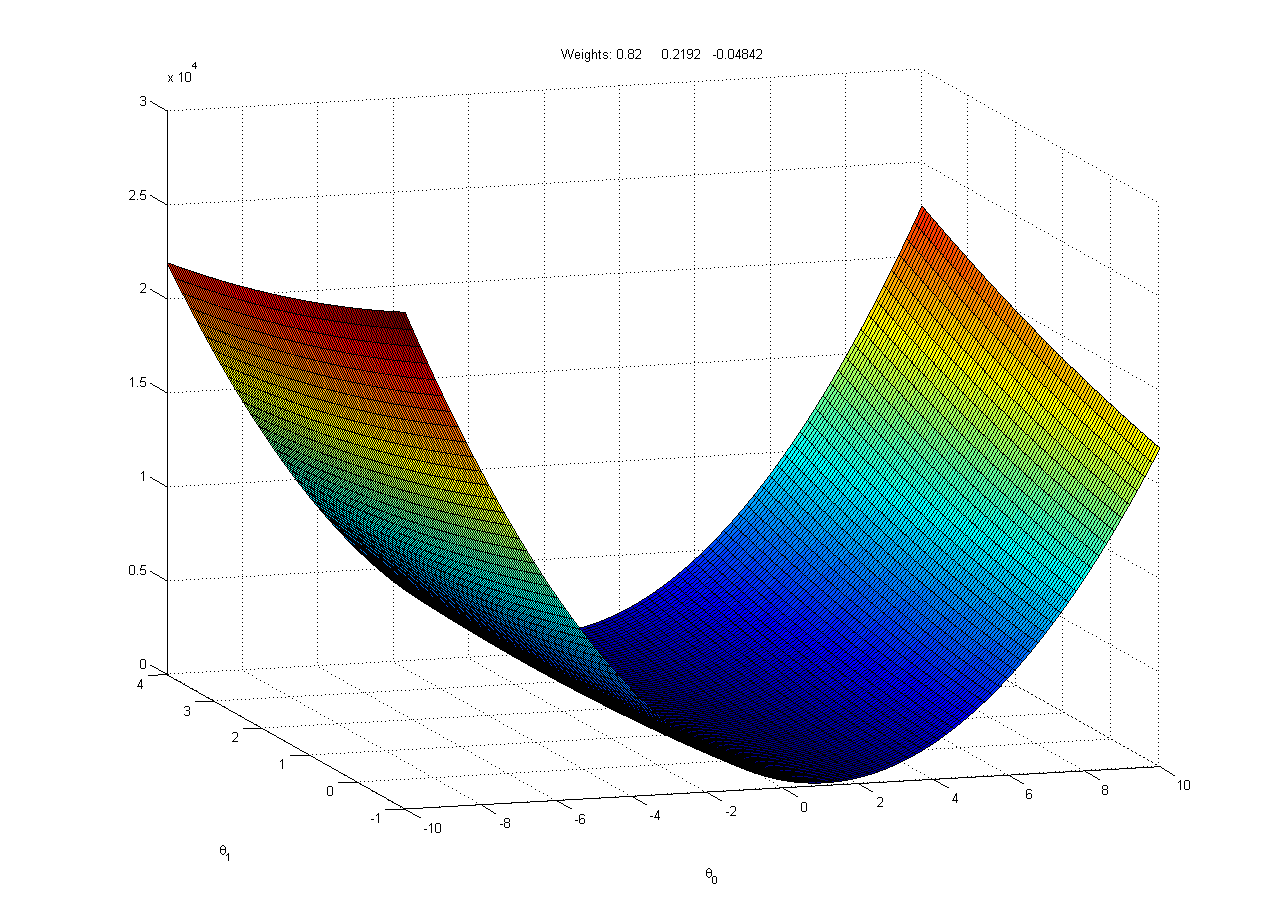
\includegraphics[width=0.5\linewidth]{lab1/linearsurf.png}
    \label{fig:linear1:sub3}
}
\caption{One layer neural network tests runs}
\end{figure}

When we modify the learning rate for the network we find that smaller learning rate means that the network takes longer to converge which inturn means that we will need more epochs before it converges. A larger learning rate has it's own problems though. A too large learning rate will make the weight matrix contain too large numbers for Matlab to be able to handle it. A slightly larger learning rate may however cause the seperating line to oscillate although it still finds the minimum.

\begin{figure}[h!]
\subfigure[The movement of the seperating line to it's final position.]{
    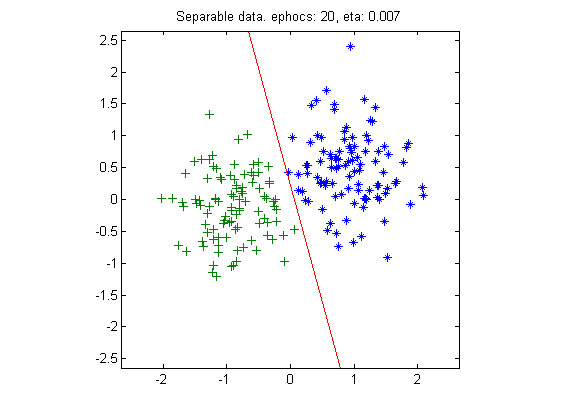
\includegraphics[width=0.5\linewidth]{lab1/linearseplargeeta.png}
    \label{fig:linear2:sub1}
}
\subfigure[The error function we're minmizing with the delta rule.]{
    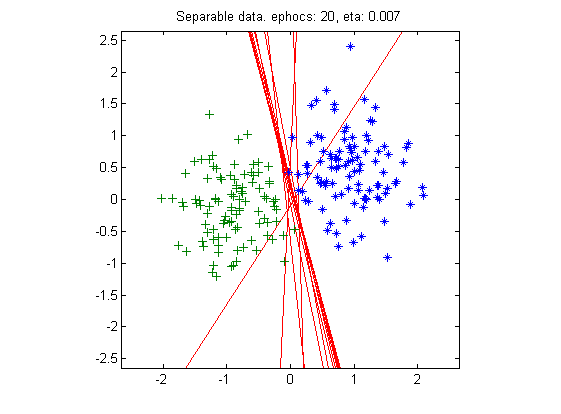
\includegraphics[width=0.5\linewidth]{lab1/linearseplargeetaall.png}
    \label{fig:linear2:sub2}
}
\caption{Larger eta values cause the weights to oscillate}
\end{figure}

Next we look at nonseperable data to see what happens. It can be seen in figure \ref{fig:linear3:sub1} and as we can see it doesn't really manage to seperate the data even though it has minimized it's error. In \ref{fig:linear3:sub2} we can see how it converged to it's final value.

\begin{figure}[h!]
\subfigure[The movement of the seperating line to it's final position.]{
    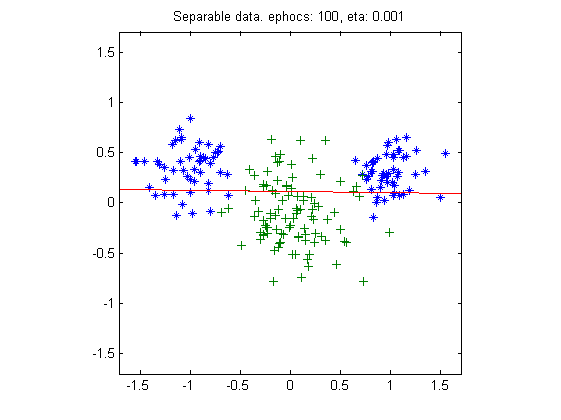
\includegraphics[width=0.5\linewidth]{lab1/linearnonsep.png}
    \label{fig:linear3:sub1}
}
\subfigure[The error function we're minmizing with the delta rule.]{
    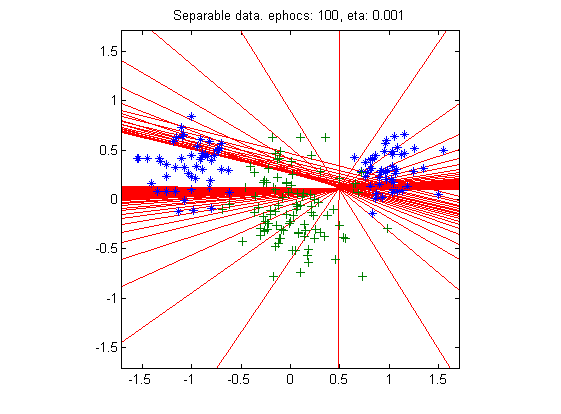
\includegraphics[width=0.5\linewidth]{lab1/linearnonsepall.png}
    \label{fig:linear3:sub2}
}
\caption{With non-seperable data the weights still converge but we don't get a good classifer.}
\end{figure}

\clearpage
\section{Two layered neural network with backprop}

Next we do the backprop algorithm for a two layer network network. The layout of the two layer network can be seen in figure \ref{fig:twolay1}.

\vspace{5cm}
\begin{figure}[h!]
\label{fig:twolay1}
\caption{The two layer neural network layout}
\end{figure}

Next we check how many nodes we need to seperate non linearly seperable data with the two layer network. The results for the euclidean error and the error of missclassified instances can be seen in figure \ref{fig:twolay2:sub2} and figure \ref{fig:twolay2:sub3}. We can see that as the number of nodes increase both error types are decreasing. It's however really difficult to actually classify all the nodes correctly and we need about 3000 nodes to classify all nodes correctly most of the time.

\begin{figure}[h!]
\subfigure[Non seperable data to run twolayer network on.]{
    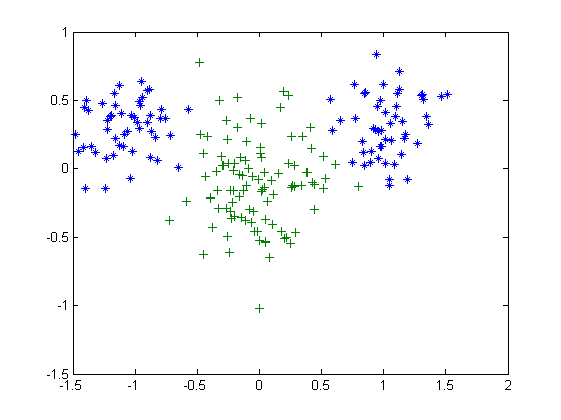
\includegraphics[width=0.5\linewidth]{lab1/twolayernonsepdata.png}
    \label{fig:twolay2:sub1}
}
\subfigure[Eucledian error for different amount of nodes.]{
    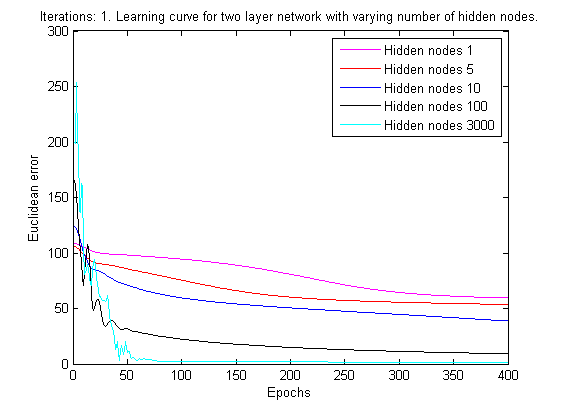
\includegraphics[width=0.5\linewidth]{lab1/twolayererrornodes.png}
    \label{fig:twolay2:sub2}
}
\subfigure[Missclassified instances for different amount of nodes.]{
    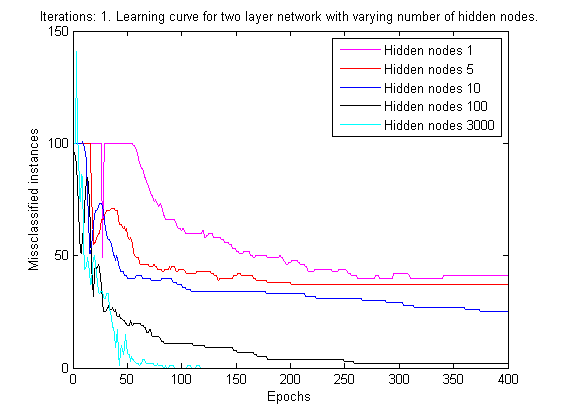
\includegraphics[width=0.5\linewidth]{lab1/twolayererrornodesclassified.png}
    \label{fig:twolay2:sub3}
}
\caption{Two layer nodes variation}
\end{figure}

Next we see how the learning rate and momentum impacts the two layer networks learning curve. We see that a highereta means a faster convergance and we also see that a too high or too low momentum makes the weights unstable and causes them to oscillate.

\begin{figure}[h!]
\subfigure[Eta change for two layer network.]{
    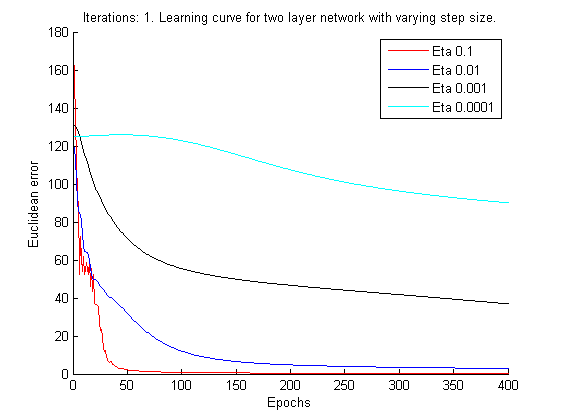
\includegraphics[width=0.5\linewidth]{lab1/twolayereta.png}
    \label{fig:twolay3:sub1}
}
\subfigure[Momentum affect on the two layer network.]{
    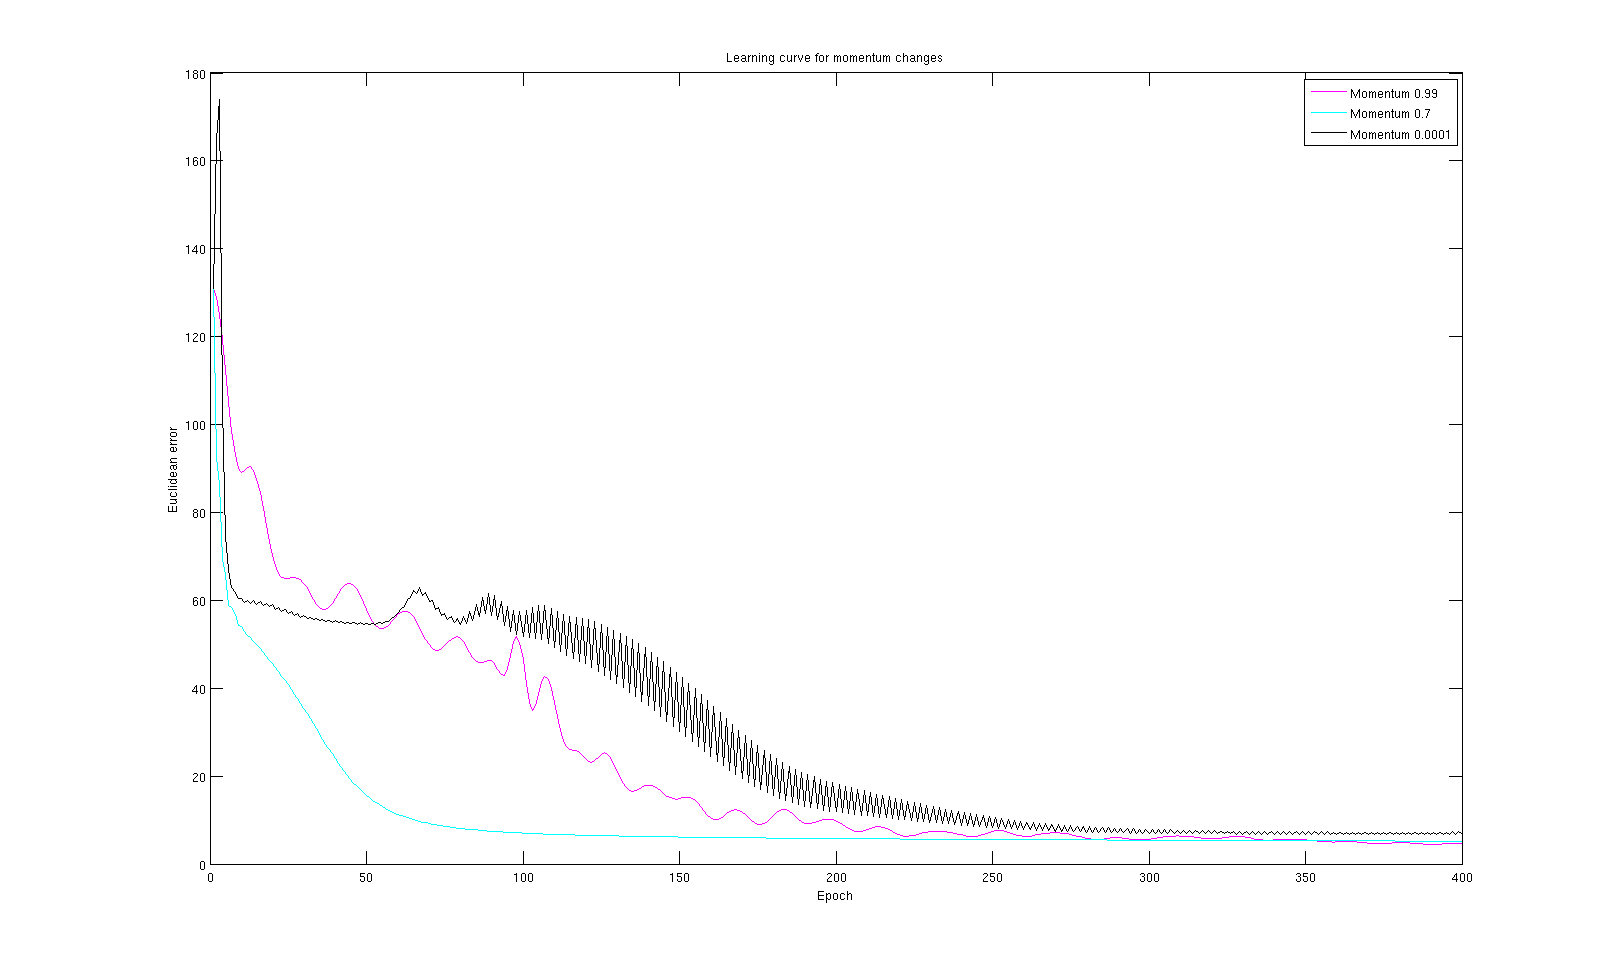
\includegraphics[width=0.5\linewidth]{lab1/twolayermomentum.png}
    \label{fig:twolay3:sub2}
}
\caption{With non-seperable data the weights still converge but we don't get a good classifer.}
\end{figure}

\clearpage
\section{Two layered neural network used for compression}
Now we will show how two layered networks can be used for datacompression. In figure \ref{fig:compress} you can see how the neural network looks for compression. For compression the output equals the input, i.e. $O=X$. In figure \ref{fig:compress2} we can see that $WX$, the compressed version of X, can be binary coded with three nodes since we have eight patterns.

\vspace{5cm}
\begin{figure}[h!]
\label{fig:compress}
\caption{The two layer neural network layout}
\end{figure}

\begin{figure}[h!]
\begin{lstlisting}
O =
     1    -1    -1    -1    -1    -1    -1    -1
    -1     1    -1    -1    -1    -1    -1    -1
    -1    -1     1    -1    -1    -1    -1    -1
    -1    -1    -1     1    -1    -1    -1    -1
    -1    -1    -1    -1     1    -1    -1    -1
    -1    -1    -1    -1    -1     1    -1    -1
    -1    -1    -1    -1    -1    -1     1    -1
    -1    -1    -1    -1    -1    -1    -1     1


WX =
    -1    -1     1    -1     1    -1     1     1
    -1     1    -1     1    -1    -1     1     1
    -1     1     1    -1    -1     1     1    -1
\end{lstlisting}
\label{fig:compress2}
\caption{Results from compression network}
\end{figure}

\clearpage
\section{Two layered neural network used for approximation}
We try and approximate a Gaussian function using a twolayered network. The result can be seen in figure \ref{fig:gauss1}.

\begin{figure}[h!]
\subfigure[Approximated gaussian function.]{
    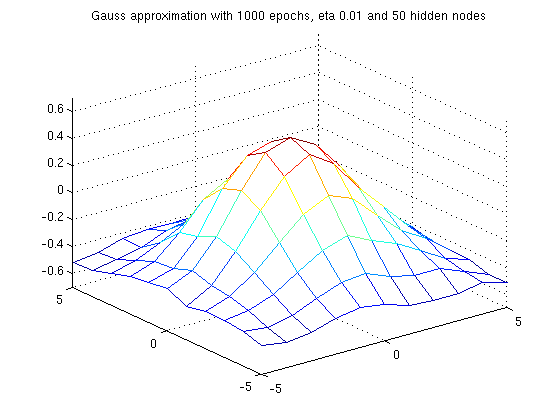
\includegraphics[width=0.5\linewidth]{lab1/gaussapprox.png}
    \label{fig:gauss1:sub1}
}
\subfigure[The real gaussian function.]{
    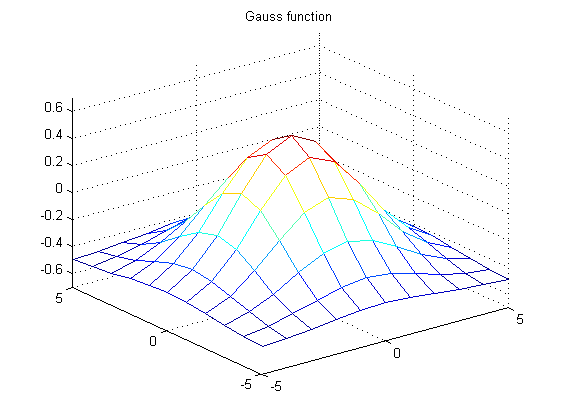
\includegraphics[width=0.5\linewidth]{lab1/gaussfunc.png}
    \label{fig:gauss1:sub2}
}
\subfigure[Non seperable data to run twolayer network on.]{
    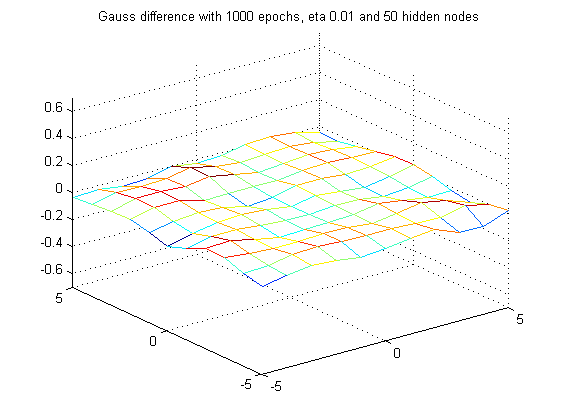
\includegraphics[width=0.5\linewidth]{lab1/gaussdiff.png}
    \label{fig:gauss1:sub3}
}
\label{fig:gauss1}
\caption{Two layer approximation of Gaussian function.}
\end{figure}

\clearpage
\section{Two layered neural network used for generalisation}

\end{document}
